\documentclass[french]{beamer}%[10pt, c, a4]
\usepackage[utf8]{inputenc}%latin1
\usepackage[frenchb]{babel}
\usepackage[T1]{fontenc}
\usepackage{graphicx}
\usepackage{pgfpages}
\usepackage{listings}
\usepackage{verbatim}
\usetheme{Antibes}
\title{Qualité logicielle}
\setbeamertemplate{footline}[frame number]
\graphicspath{{images/}}

\author[Abderrahim El Jaouhary, Frédéric Malard]
{
	Abderrahim El Jaouhary, Frédéric Malard \\\medskip
	{\small \nolinkurl{}{codeligne@gmail.com}} \\ 
	{\small \nolinkurl{fred.malard2@gmail.com}}
}

\AtBeginSection[]
{
  \begin{frame}[shrink]{Plan}
  \small \tableofcontents[currentsection,hideothersubsections]
  \end{frame} 
}

\begin{document}
	
	\begin{frame}
		\titlepage
	\end{frame}
	
	\begin{frame}[shrink]{\secname}
	    \tableofcontents[subsectionstyle=hide]
	\end{frame}
	
	\section{introduction}
		
		\begin{frame}
			\begin{itemize}
			    \item Définition
			    \item Historique
			    \item Documentation et tests
			\end{itemize}
		\end{frame}
		
	\section{Indicateurs}
		
		\subsection{norme 9126}
		
			\begin{frame}
				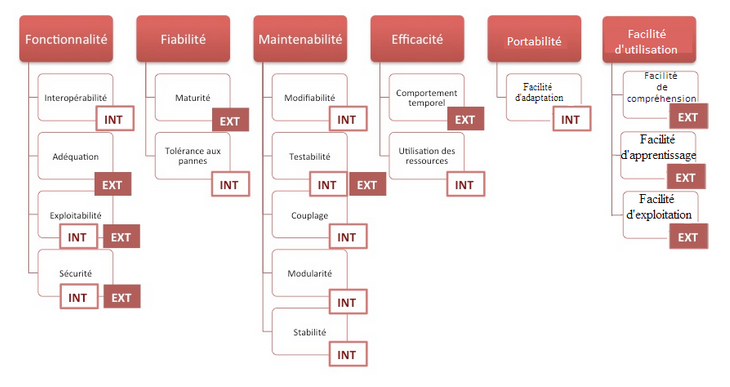
\includegraphics[scale = 0.4]{indicateurs.jpg}
				\newline
				Fonctionnalité : le logiciel répond t-il aux besoins fonctionnels exprimés ?
			\end{frame}
			
			\begin{frame}
				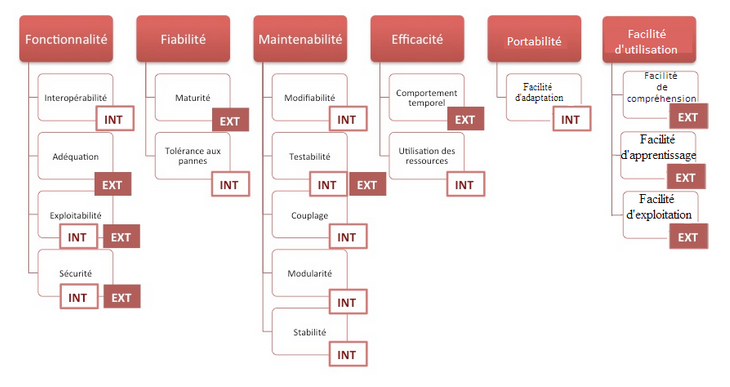
\includegraphics[scale = 0.4]{indicateurs.jpg}
				\newline
				Fiabilité : conditions et durées du maintient du niveau de service
			\end{frame}
			
			\begin{frame}
				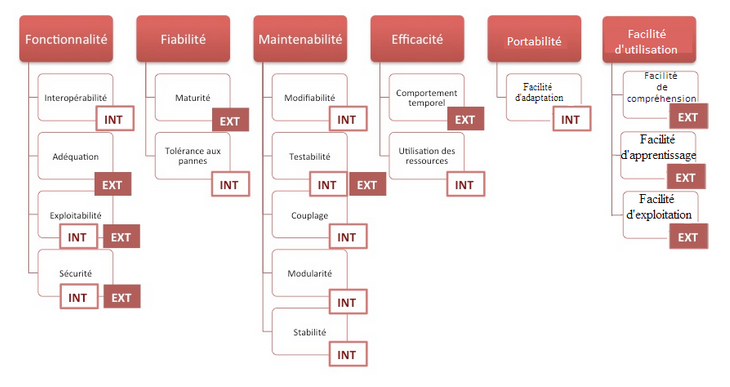
\includegraphics[scale = 0.4]{indicateurs.jpg}
				\newline
				Maintenabilité : aisance a la correction et a la modification des fonctionnalités
			\end{frame}
			
			\begin{frame}
				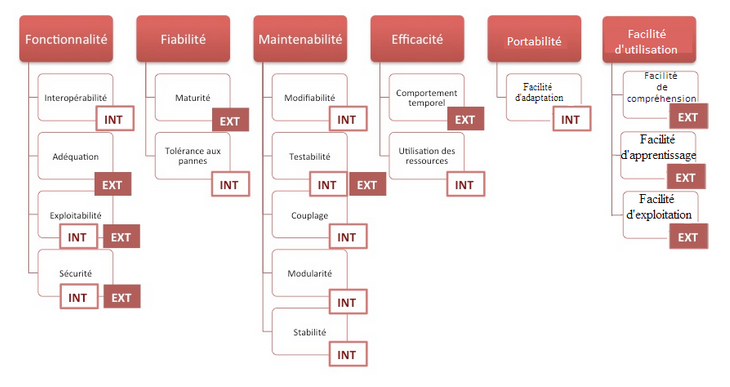
\includegraphics[scale = 0.4]{indicateurs.jpg}
				\newline
				Efficacité : résultats obtenus / ressources exigées
			\end{frame}
			
			\begin{frame}
				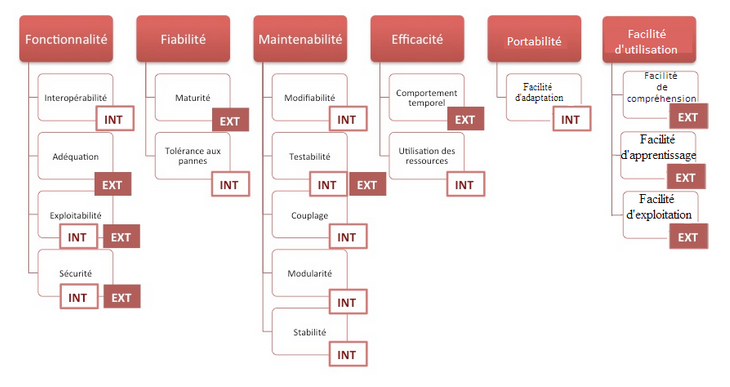
\includegraphics[scale = 0.4]{indicateurs.jpg}
				\newline
				Portabilité : aisance a transférer le logiciel d'un environnement a un autre
			\end{frame}
			
			\begin{frame}
				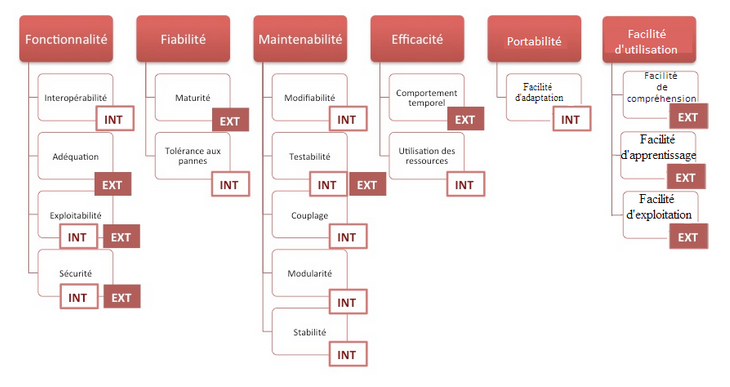
\includegraphics[scale = 0.4]{indicateurs.jpg}
				\newline
				Facilité d'utilisation : aisance a prendre en main le logiciel pour un nouvel utilisateur
			\end{frame}
			
		\subsection{norme SCOPE}
			
			\begin{frame}
				\begin{center}
					\begin{figure}
						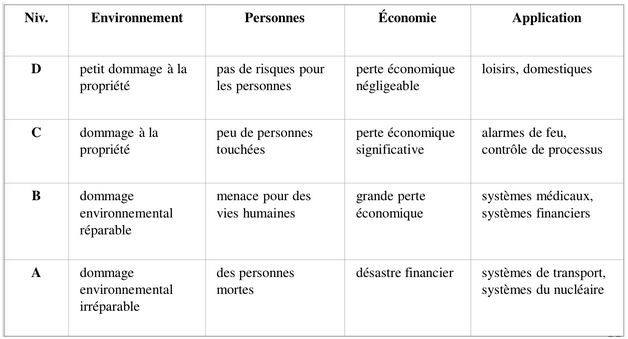
\includegraphics[scale = 0.5]{scope1}
						\caption{SCOPE}
					\end{figure}
				\end{center}
			\end{frame}
			
			\begin{frame}
				\begin{center}
					\begin{figure}
						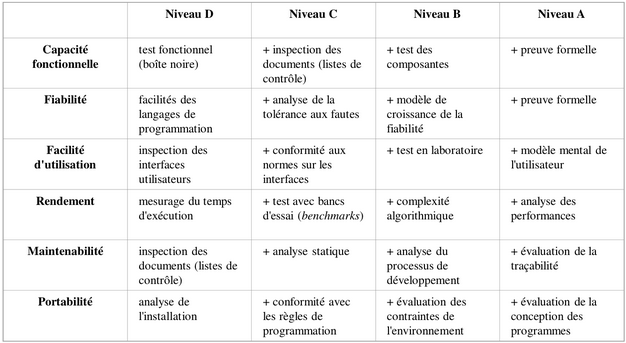
\includegraphics[scale = 0.5]{scope2}
						\caption{SCOPE}
					\end{figure}
				\end{center}
			\end{frame}
			
	\section{Mesure}
		
		\subsection{indice de spécialisation}
		
			\begin{frame}
				\begin{center}
					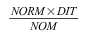
\includegraphics[scale=1]{speFormule}
					\newline
					NORM = nombre de méthodes redéfinies
					\newline
					DIT = profondeur de la classe dans l'arbre d'héritage
					\newline
					NOM = nombre de méthodes de la classe
				\end{center}
			\end{frame}
		
			\begin{frame}
				\begin{center}
					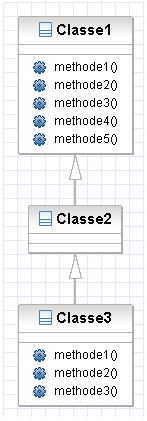
\includegraphics[scale=0.4]{speGraph1}
				\end{center}
			\end{frame}
		
			\begin{frame}
				\begin{center}
					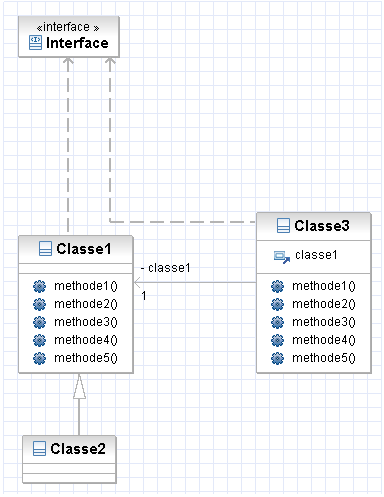
\includegraphics[scale=0.35]{speGraph2}
				\end{center}
			\end{frame}
		
		\subsection{incide d'instabilité}
		
			\begin{frame}
				\begin{center}
					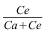
\includegraphics[scale=1]{instFormule}
					\newline
					Ce = couplage efferent
					\newline
					Ca = couplage afferent
				\end{center}
			\end{frame}
		
			\begin{frame}
				\begin{center}
					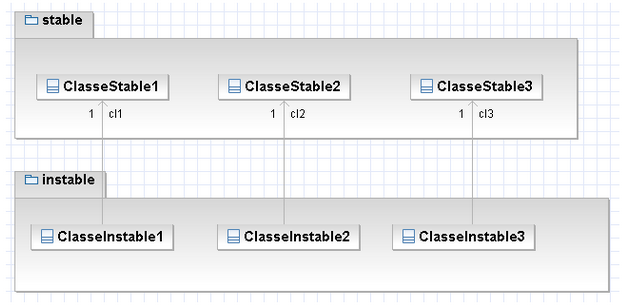
\includegraphics[scale=0.45]{instGraph}
				\end{center}
			\end{frame}
		
		\subsection{complexité cyclomatique}
		
			\begin{frame}
				\begin{center}
					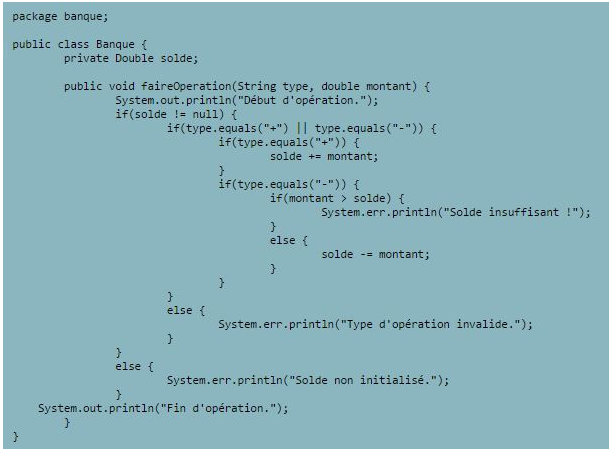
\includegraphics[scale=0.4]{cycloCode}
				\end{center}
			\end{frame}
		
			\begin{frame}
				\begin{center}
					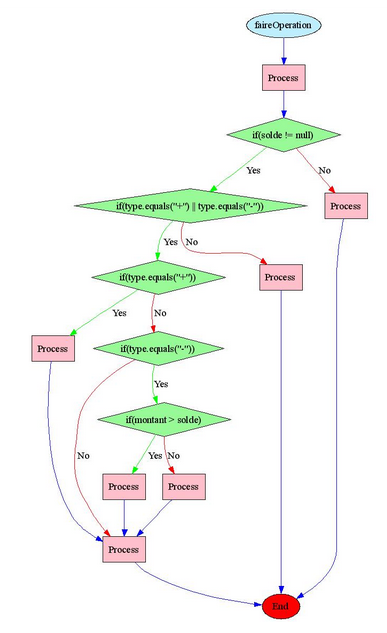
\includegraphics[scale=0.3]{cycloGraph}
				\end{center}
			\end{frame}
			
	\section{bonnes manières de coder}
	
		\subsection{MVC}
		
			\begin{frame}
				\begin{center}
					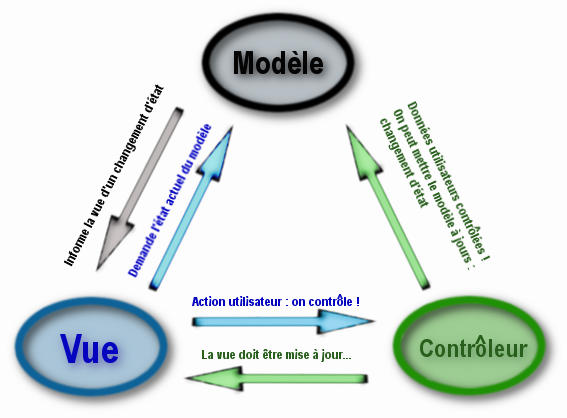
\includegraphics[scale=0.3]{MVCschema}
				\end{center}
			\end{frame}
	
		\subsection{algorithmique}
		
			\begin{frame}
				\begin{center}
					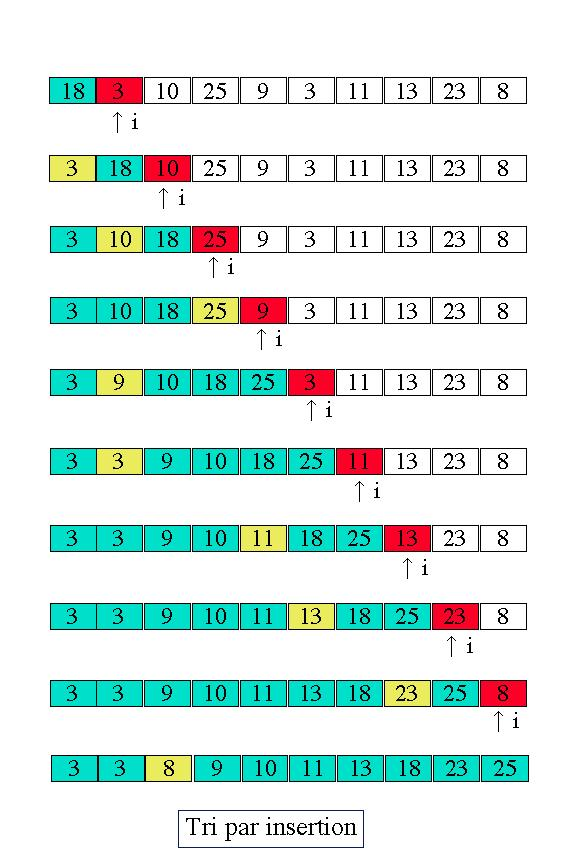
\includegraphics[scale=0.22]{TIS}
				\end{center}
			\end{frame}
		
			\begin{frame}
				\begin{center}
					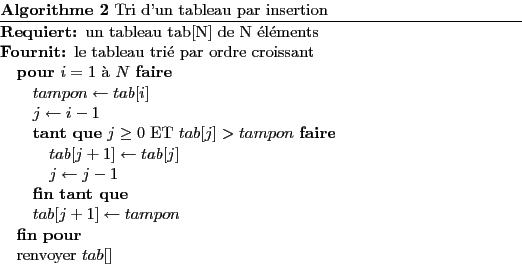
\includegraphics[scale=0.5]{TIC}
				\end{center}
			\end{frame}
		
			\begin{frame}
				\begin{center}
					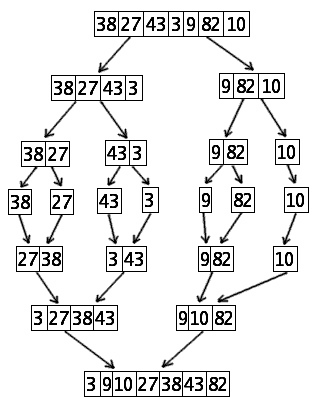
\includegraphics[scale=0.4]{TFS}
				\end{center}
			\end{frame}
		
			\begin{frame}
				\begin{center}
					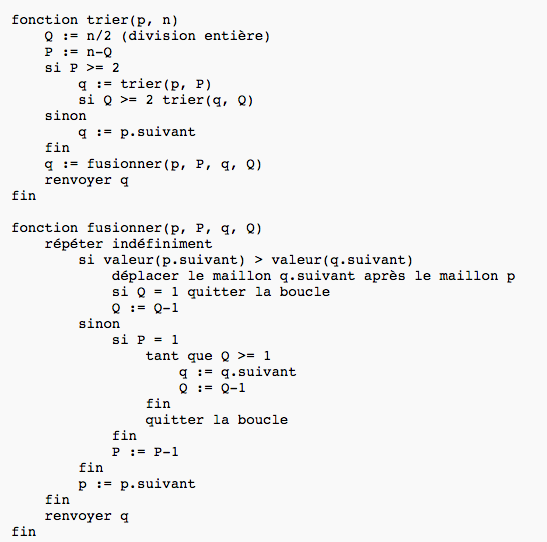
\includegraphics[scale=0.35]{TFC}
				\end{center}
			\end{frame}
	
		\subsection{exceptions}
		
			\begin{frame}
				\begin{center}
					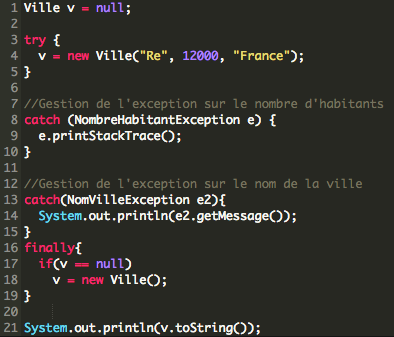
\includegraphics[scale=0.5]{exceptions}
				\end{center}
			\end{frame}
	
		\subsection{factorisation}
		
			\begin{frame}
				\begin{itemize}
					\item fonctions
					\item classes
					\item héritage
					\item macros
					\item et bien d'autres techniques
				\end{itemize}
			\end{frame}
	
		\subsection{portabilité}
		
			\begin{frame}
				\begin{center}
					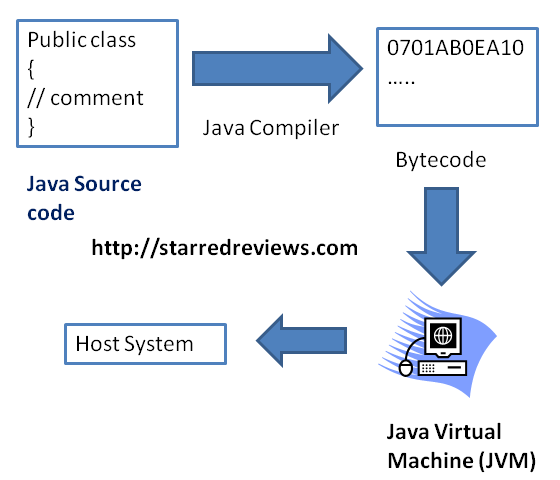
\includegraphics[scale=0.5]{JVM}
				\end{center}
			\end{frame}
	
		\subsection{UML}
		
			\begin{frame}
				\begin{center}
					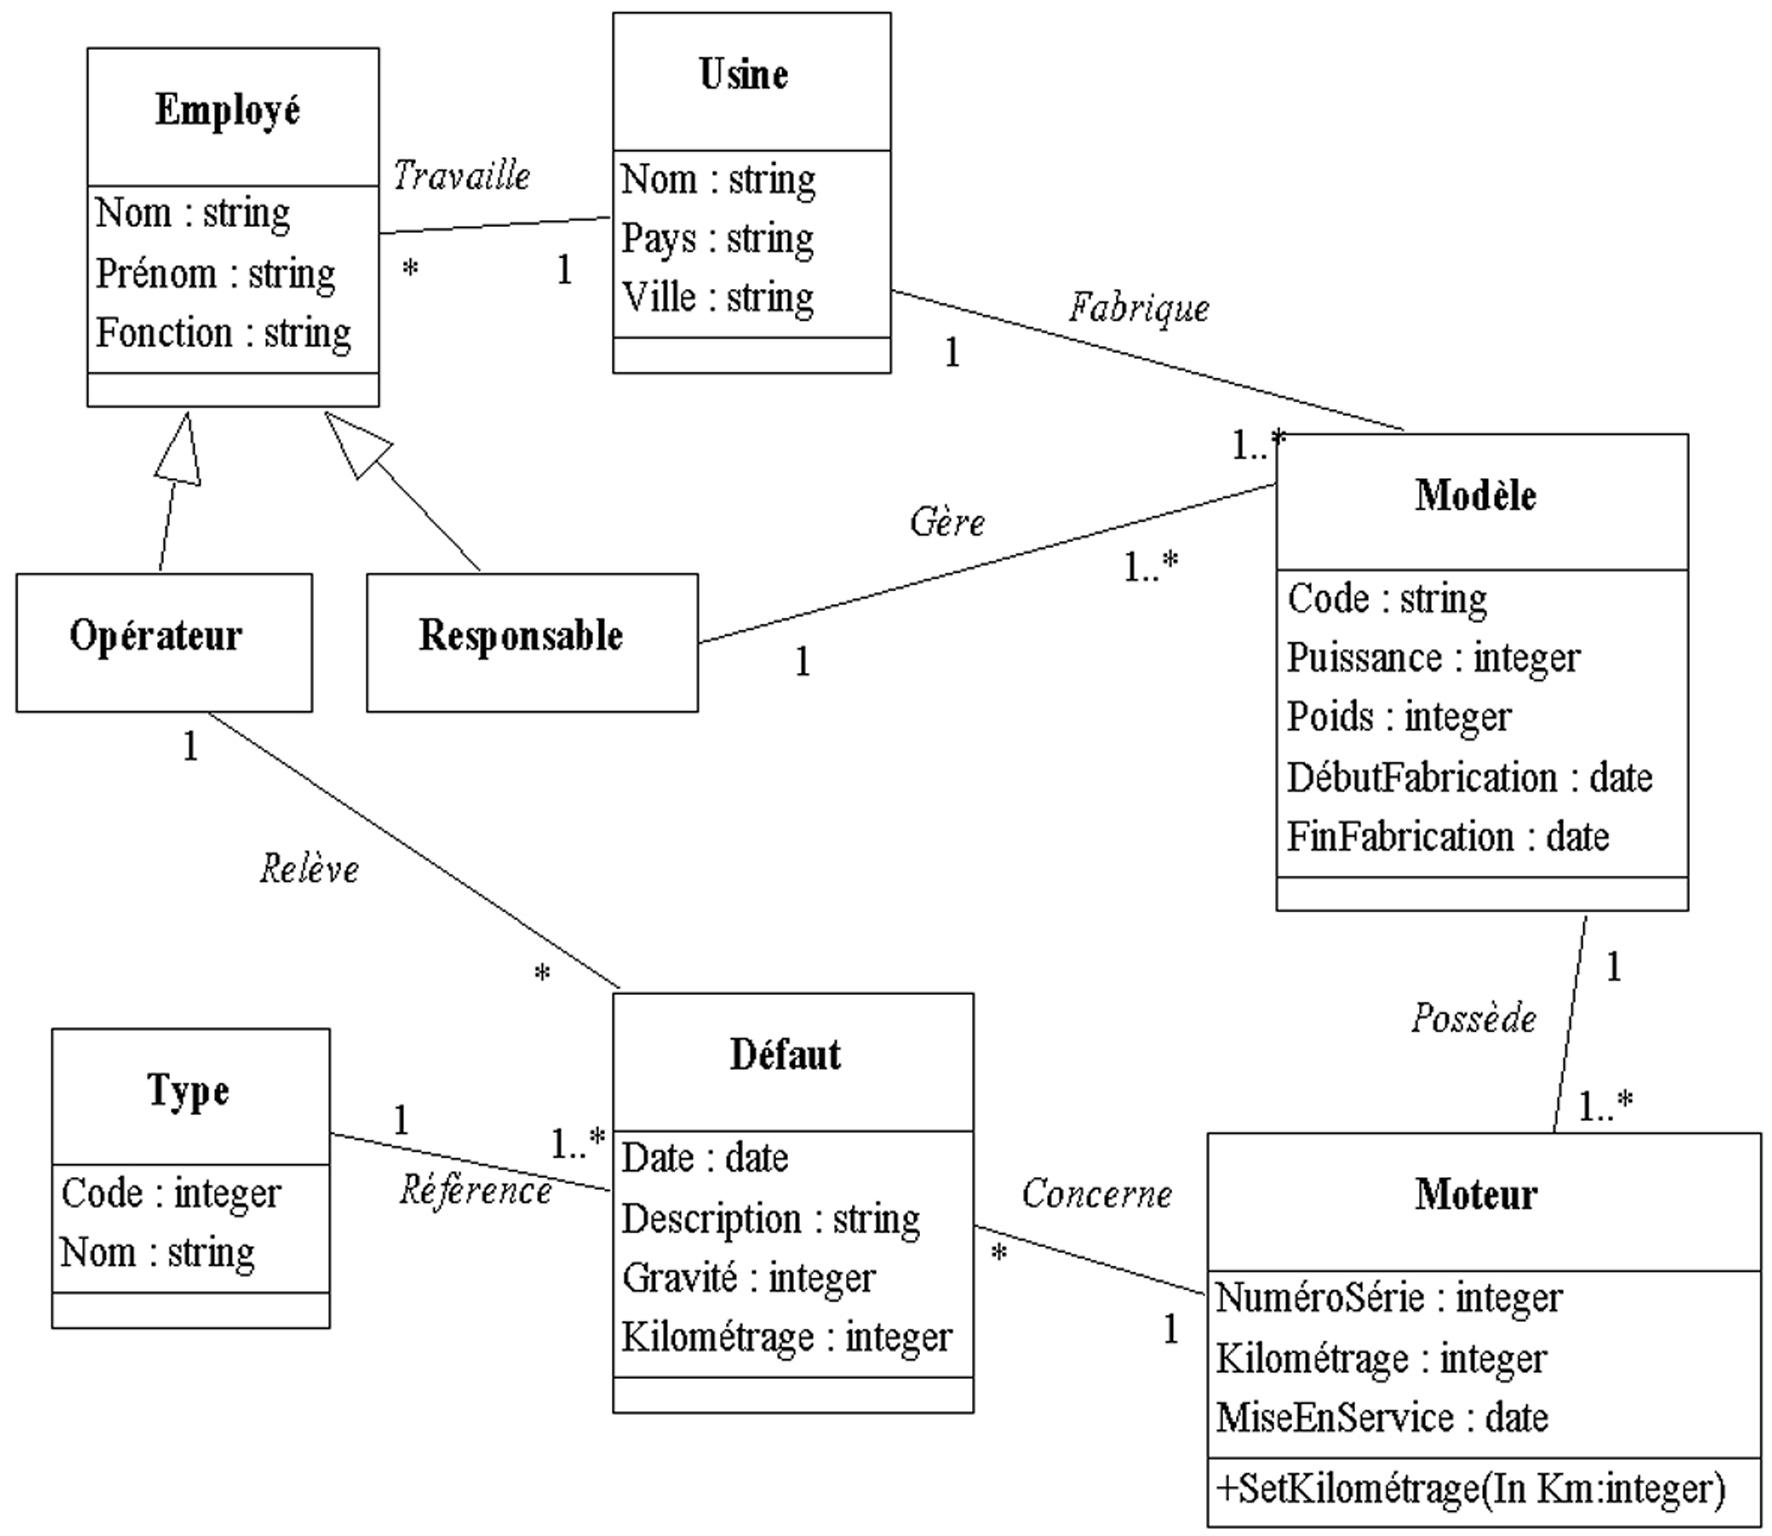
\includegraphics[scale=0.13]{UML}
				\end{center}
			\end{frame}
	
		\subsection{et bien d'autres}
	
			\begin{frame}
				\begin{itemize}
					\item IHM (interfaces homme-machine)
					\item commentaires
					\item code propre
					\item etc.
				\end{itemize}
			\end{frame}
	
\end{document}